\documentclass[11pt,a4paper]{article}

\usepackage{graphicx}
\usepackage{url}
\title{Interface IO port expander with R-Pi}
\author{e-Yantra Team}
\date{\today}

\begin{document}
	\maketitle
	\newpage
	\tableofcontents
	\newpage
	\section{Objective}
	In this tutorial we will learn how to interface a port expander i.e. MCP23017 IC with an R-Pi to increase the number of input/output pins.
	\section{Prerequisites}
	One should have:
	\begin{itemize}
		\item Python programming skills
		\item Some knowledge about performing basic programs to access GPIO pins of an R-Pi
		\item Some basic information regarding different serial communication \newline protocols
	\end{itemize}
	\section{Hardware Requirement}
	\begin{enumerate}
		\item Raspberry Pi (I will be using Version 2 Model B)
		\item Power adapter
		\item MCP23017 IC
		\item Connecting wires
		\item Bread board
	\end{enumerate}
	\section{Software Requirement}
	MobaXterm (for windows user) 
	
	\newpage
	\section{Theory and Description}
	The no. of GPIO pins in an R-Pi is less(merely 26 in R-Pi 2) and so interfacing sensors and other modules would consume most of the pins thus setting a limit for I/O access. Therefore in order to increase the no. of GPIO pins we can interface a port expander to an R-Pi.
	
	A port expander is a hardware device designed to allow a user to utilize more than one device on a single port at one time. For example, the device may allow seven devices to connect to one serial port.[1]
	
	\subsection{I2C}
	I²C (Inter-Integrated Circuit), pronounced I-squared-C, is a multi-master, multi-slave, single-ended, serial computer bus used for attaching lower-speed peripheral ICs to processors and micro controllers.[2]
	
	The two I²C signals are called 'serial data’ (SDA) and ‘serial clock’ (SCL). There is no need of chip select (slave select) or arbitration logic in this. Virtually any number of slaves and any number of masters can be connected onto these 2 signal lines and communicate between each other using a protocol that defines:
	\begin{itemize}
			\item 7-bits slave addresses: each device connected to the bus has got such a unique address
			\item data divided into 8-bit bytes
			\item a few control bits for controlling the communication start, end, direction and for an acknowledgement mechanism.
	\end{itemize}

	The data rate has to be chosen between 100 kbps, 400 kbps and 3.4 Mbps, respectively called standard mode, fast mode and high speed mode. Some I²C variants include 10 kbps (low speed mode) and 1 Mbps (fast mode +) as valid speeds.
	
	Physically, the I²C bus consists of the 2 active wires SDA and SCL and a ground connection. The active wires are both bi-directional.[3] 
	\begin{figure}[h!]
		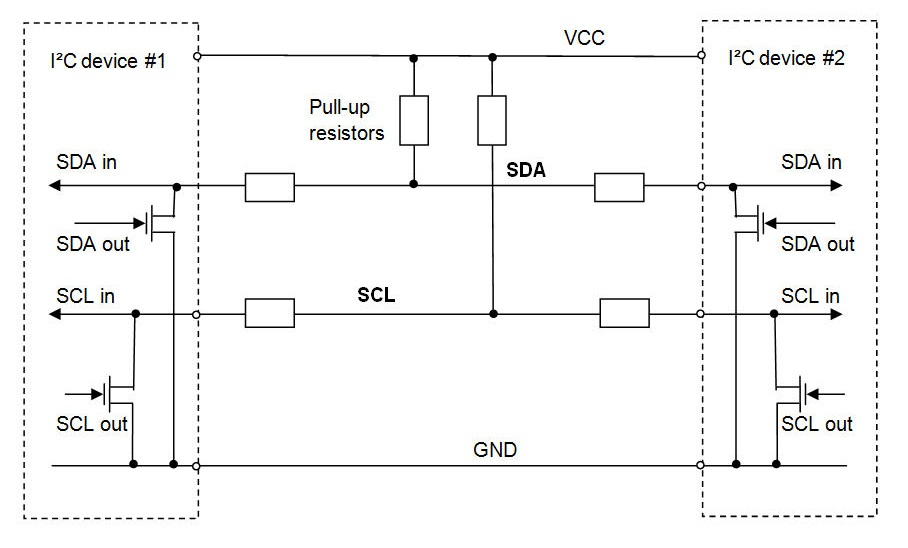
\includegraphics[scale=0.4]{i2c.jpg}
		\centering
		\caption{[3]}
	\end{figure} 
	
	\newpage
	The I2C protocol specification states that the IC that initiates a data transfer on the bus is considered the Bus Master. Consequently, at that time, all the other ICs are regarded to be Bus Slaves. 
	
	\flushleft
	\textbf{Data transfer using I2C}
	\begin{enumerate}
		\item First, the master will issue a START condition. This acts as an ‘Attention’ signal to all of the connected devices. All ICs on the bus will listen to the bus for incoming data.
		\item Then the master sends the ADDRESS of the device it wants to access, along with an indication whether the access is a Read or Write operation. Having received the address, all IC’s will compare it with their own address. If it doesn’t match, they simply wait until the bus is released by the stop condition. If the address matches, however, the chip will produce a response called the ACKNOWLEDGE signal.
		\item Once the master receives the acknowledgement, it can start transmitting or receiving DATA.When all is done, the master will issue the STOP condition. This is a signal that states the bus has been released and that the connected ICs may expect another transmission to start any moment.
		\item When a master wants to receive data from a slave, it proceeds the same way, but sets the R/W bit at a logical one. Once the slave has acknowledged the address, it starts sending the requested data, byte by byte. After each data byte, it is up to the master to acknowledge the received data.[3]
	\end{enumerate}
	
	\subsection{Enabling I2C interface on R-Pi}
	\begin{enumerate}
		\item Open MobaXterm then open LXTerminal(if using LXDE desktop) else on the terminal window type \textit{sudo nano /etc/modules}
		\item A file opens, add the following two lines to the end of the file: \textit{i2c-bcm2708 } and  \textit{i2c-dev}. Then save the file by Ctrl+X , Y.
		\begin{figure}[h!]
			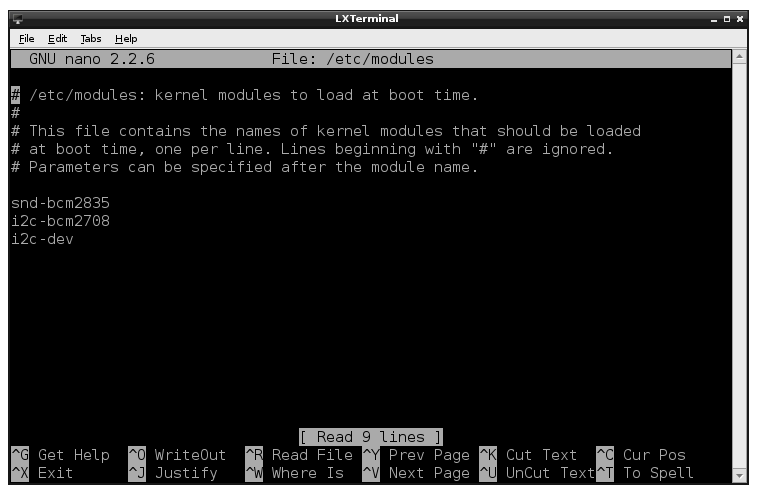
\includegraphics[width=11cm]{1.png}
			\centering
			\caption{[4]}
		\end{figure} 
		\item In case you have a file called \textit{/etc/modprobe.d/raspi-blacklist.conf} then edit the file as shown below(comment the 2 lines)
		\newpage
		\begin{figure}[h!]
			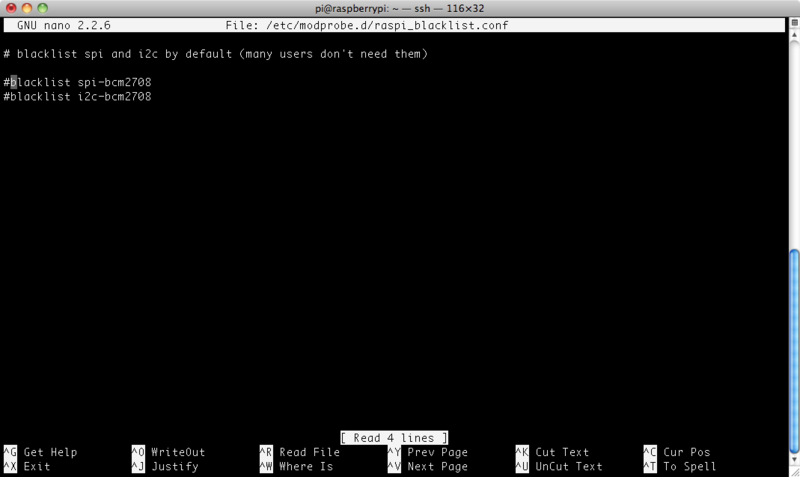
\includegraphics[scale=0.4]{2.png}
			\centering
			\caption{[4]}
		\end{figure}
		\textbf{Note:} In case you don't have this file continue with the further steps.
		
		\item Recent versions of Raspberry Pi need an update to\textit{/boot/config.txt} file. Type the command \textit{sudo nano /boot/config.txt} and edit the file by adding the following two lines at the end of the file: \textit{dtparam\=i2c1\=on} and \textit{dtparam\=i2c\_arm\=on}
				
		\item After all this is done reboot the system by using the command \textit{sudo reboot}	
	
	\end{enumerate}
	
	\newpage
	\subsection{MCP23017}
	It is a 16 bit I/O expander with serial interface. Some of its features are:
	\begin{itemize}
		\item 16-bit remote bidirectional I/O port (I/O pins default to input)
		\item High-speed I2C interface (100 kHz, 400 kHz, 1.7 MHz)
		\item Three hardware address pins to allow up to eight devices on the bus
		\item Two pins to communicate with a master controller i.e. SCL and SDA
	\end{itemize}
	
	\begin{figure}[h!]
		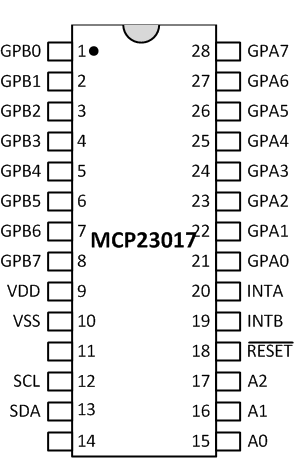
\includegraphics[scale=0.7]{mcp23017.png}
		\centering
		\caption{[5]}
	\end{figure}
	
	\flushleft
	For further information you refer the Appendix section.
	
	\newpage
	\section{Experiment}
	In order to start programming the port expander(MCP23017) , we need to interface the IC with R-Pi in the following way:
	\begin{figure}[h!]
		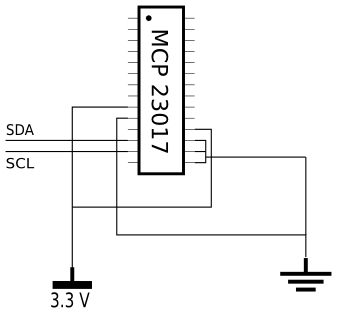
\includegraphics[scale=0.8]{interface.png}
		\centering
		\caption{[6]}
	\end{figure} 
	\flushleft
	
	\begin{itemize}
		\item Connect the VDD pin and RESET on MCP23017 to 3.3v pin on an R-Pi 
		\item Connect the VSS pin on MCP23017 and A0,A1,A2 pin to GND pin on an R-Pi(If you are using 1 port expander IC then we connect the 3 address pins A0, A1 and A2 pins to GND)
        \item Connect the SCL and SDA pins from the MCP23017 IC to the respective pins on R-Pi
	\end{itemize}
	
	\vspace{0.3cm}
	\textbf{Please refer the Appendix section before making the necessar connections. }
	
	\vspace{0.3cm}
	After making all the necessary connections type the following command on the terminal \textit{sudo i2cdetect -y 1} (to see the device addresses of MCP23017 IC's interfaced )
		
	\vspace{0.3cm}
	\textbf{Note :} For a version 1 R-Pi with RAM lesser than 512MB use the command \textit{sudo i2cdetect -y 1} 
	
	\newpage

	\section{Appendix}
	\subsection{Raspberry Pi 2 Pin-out Diagram}
	\begin{figure}[h!]
		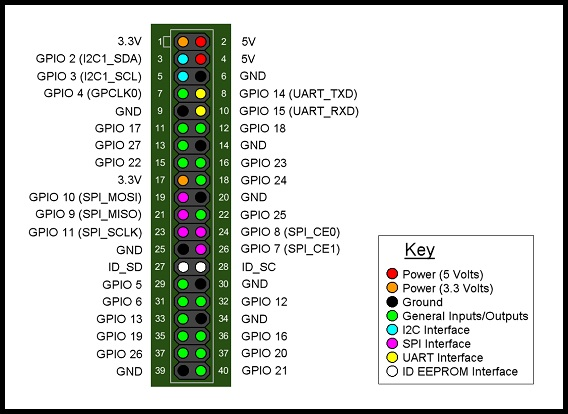
\includegraphics[scale=0.6]{RaspberryPi2_pinout.jpg}
		\centering
		\caption{[7]}
	\end{figure}
	
	\subsection{MCP23017 datasheet}
	
	\url{http://ww1.microchip.com/downloads/en/DeviceDoc/21952b.pdf}
	
	\newpage
    \section{References}
    \begin{enumerate}
    	\item \url{http://www.computerhope.com/jargon/p/portexpa.htm}
    	\item \url{https://en.wikipedia.org/wiki/I%C2%B2C}
    	\item \url{http://www.byteparadigm.com/applications/introduction-to-i2c-and-spi-protocols/}
    	\item \url{https://learn.adafruit.com/adafruits-raspberry-pi-lesson-4-gpio-setup/configuring-i2c}
    	\item \url{https://www.mathworks.com/examples/matlab/4547-add-digital-i-o-pins-to-raspberry-pi-hardware-using-mcp23017}
    	\item \url{https://camo.githubusercontent.com/c80be3d0c9e3146cd09e15b7ddf07dbb8b7d40b8/687474703a2f2f692e696d6775722e636f6d2f4575524e722e706e67}
    	\item \url{http://data.designspark.info/uploads/images/53bc258dc6c0425cb44870b50ab30621}
    \end{enumerate}
    
\end{document}



